\chapter{Introduction}\label{chap:Intro}

\section{Motivation}

Zebrafish has recently emerged as an invaluable model for biomedical research. Enormous amounts of data is being generated from imaging zebrafish embryos. Manual image analysis is cumbersome and subjective, there by increasing the need for automated image analysis tools. Lack of automated image processing tools for zebrafish analysis is a huge bottleneck in realizing zebrafish application to its full potential.

\par
The growing utility of zebrafish as a model for biomedical research is attributed to its properties such as transparency, reproducibility, growth rate, and small size. The transparency of zebrafish embryo makes it a good model for direct observation of the development of organs and tissue. For this reason, zebrafish has been widely utilized to study neural developmental \cite{campbell2006}, and vasculature development \cite{fouquet1997}. It enables researchers to study different development stages of zebrafish to adulthood \cite{Kimmel95}. Transparent zebrafish promotes relatively easy modification of genetic expressions to mimic various diseases including Cancer \cite{Amatruda08}, Alzheimer \cite{Newman11}, and Parkinsons \cite{Boehmler09}. Neuronal structures and blood vessels can be directly observed, providing an opportunity to study abnormal neuronal and vascular patterns due to gene manipulation, drug screening and other environmental cues.

\par
Its small size and high reproduction rate allows researchers to image a large number of zebrafish in a short period of time \cite{Leonard05}. Advantages of zebrafish as a vertebrate animal model make it suitable for screening chemicals in an effective manner \cite{Kaufman09}.  Studies are being conducted to evaluate the embryotoxic effect of chemicals \cite{Yang09}. Transgenic zebrafish has been developed to  study the effects of chemicals on blood vessel development \cite{Tran07}. The availability of a large number of zebrafish embryos makes them suitable for characterizing gene expressions \cite{Fan10}. 

\par
Advances in imaging technique combined with various advantages of zebrafish, is another reason driving their wide applicability in various research areas \cite{Leonard05}. Imaging zebrafish is fast and cost-effective as compared with other animal models. Thus, zebrafish is becoming one of the most popular species in high-throughput screening. In most of the above work, data is generated in large amounts and it is difficult to analyze it manually. Manual analysis is time-consuming, suffers from inter class variability and is not scalable for high throughput analysis. With rapid advances in science and environmental pollution, the need to screen huge numbers of compounds during the drug screening and toxicology analysis has been growing. At present, there is substantial effort required to validate assays for such use. A key challenge has been the automated assessment of imaging data because there are few image analysis tools capable of performing analysis in automated manner. In the past few years, there has been a significant increase in the number of research efforts focusing on analyzing behavioral and morphological features in adult zebrafish \cite{Liu06}. Morphological analysis methods have been developed to extract features of neurons \cite{Kimmel95} and vasculatures \cite{Feng05} from zebrafish. Methods have also been developed where zebrafish swimming pattern and behavior are recorded by video equipment for analysis in response to stress, predators, alarms, and drugs \cite{Bang02}. 

In this thesis, we focus on developing image processing algorithms for segmentation, analysis, and classification of zebrafish under the influence of various chemicals. The interpretation and analysis of toxicology screens consumes about 70\% of analysis time \cite{alshut2010}. Due to industrialization, we need to regularly perform a risk assessment on new chemicals, pesticides, and drugs. Frequency with which new hazardous chemicals are being identified further emphasizes the magnitude of the problem. Concurrent with the increasing levels of environmental pollution, accumulating evidence shows that there is a vital need to study effects of exposure levels on human and animal health \cite{mccollum2014}. Research community is still trying to understand the effects of exposure of chemicals on organism. There are many questions that have to be answered. Firstly, what is the nature of effect, and to what extent? Secondly, after what dosage to study chemicals do the hazardous effects becomes threatening? Is there a way to establish predictive toxicity testing of chemicals? zebrafish as the model of toxicology has been well established. Emphasis is on creating tools for toxicity assessment through qualitative or quantitative screening for varying exposure levels of toxicants.


\section{Zebrafish Image Analysis}

Over the past several years, efforts have been dedicated to developing methods to process, analyze, and quantify zebrafish images. Over the years researchers have dedicated efforts to develop image processing algorithms to analyze behavior of zebrafish. The first step in image processing for behavioral analysis is usually the continuous tracking and segmentation of the whole zebrafish from digital images. Bang et al. developed an automated screening assay to detect hearing effects in zebrafish by monitoring their behavior after receiving a loud sound burst \cite{Bang02}. Kato et al. proposed to study swimming pattern and schooling behavior for analysis \cite{Kato04}. 

\par
Various neurobiological analysis algorithm for quantifying changes in zebrafish has been proposed. Xu at al. \cite{Xu10} proposed an algorithm focused on detecting and quantifying pigments in zebrafish embryos. They automatically identify torso area through series of image processing steps. Liu et al. \cite{Liu06} have proposed to automatically quantify the neurons and somites in a large number of zebrafish images, as well as quantitative measurement of gene expression levels in zebrafish embryos. Chen et al. \cite{Chen11} proposed a robust automatic segmentation to identify region of interest (ROI) for gene expression quantification.

\par
Image processing methods have also been developed to analyze morphological features in zebrafish. Stern et al. \cite{Stern11} focuses on automatically detecting specific interest points in microscopy images. Alshut et al. \cite{alshut2010} proposed learning based classification approach, which detects the embryo in the well, classifies its status as dead, alive or unknown, and derives characteristic parameters for the regions. Liu \cite{Liu12} proposed a recognition model for high throughput screening of toxicity based on image descriptors based on color and texture combined with a support vector machine to recognize three basic phenotypes (hatched, unhatched, and dead).

\par
In addition to neuronal structure, blood vessels is another structure that is often used in zebrafish-based studies. These studies are particularly interesting since, the cardiovascular system is one of the first organ to emerge during embryonic development. The vascular system is a vital component of all vertebrate animals, supplying oxygen and essential nutrients to every tissue and organ. Zebrafish have a closed circulatory system, and the mechanism of vessel formation are highly similar to those in humans.  A wide range of congenital diseases are associated with blood vessel formation \cite{folkman1995}, development of the cardiovascular system and associated vascular defects \cite{shalaby1995}, and the adverse effects of exposure to toxic elements during development \cite{kleinstreuer2011}. Some previous studies have already employed image processing methods to studying vasculature development. Tran et al. \cite{Tran07} proposed an algorithm using the Discovery-1/MetaMorph software to analyze blood vessel images. Vogt et al. \cite{Vogt09} implemented a user guided image interpretation tool to generate rule-based hierarchical image segmentation and blood vessels quantification. Feng et al. \cite{Feng05} developed a 3D attributed vessel representation graph (AVRG) approach to reconstruct caudal vasculature of zebrafish embryo. The whole vascular structure is reconstructed and then utilized for quantification of the number and connectivity of the vessels, their size, length, and volume, as well as the distance between any two vessels. Existing method perform well with uniformly illuminated zebrafish images, but resolve to manual analysis under varying illumination \cite{Tran07}. Automated analysis of vasculature is still a budding field. Feng et al. \cite{Feng05}, and Vogt et al. \cite{Vogt09} are the only studies dedicated to automated analysis of vasculature blood vessel. The work presented in the above mentioned has been performed on limited number of screens; there is still a question about its scalability. %Feng et al. performed 3d reconstruction of few vessels obtained using confocal microscopy, as opposed to our work we capture the dynamics of all blood vessels in same region. 

\par
In this work, we focus on developing an image processing algorithms for the high-throughput screening (HTS) of assays of compounds for toxicology analysis. In particular, we will focus on the vasculature system of zebrafish. The methodology presented in this work is quantitative, can be utilized in wide varieties of toxin treated zebrafish, and capable of quantifying changes in fine structure not quantifiable by the human eye. Based on existing methods, automatic identification of the applicable ROI, and accurate quantification of ROI features has been very challenging. 
%and review contributions made by this system to our understanding of vascular development. trying to link vasculature and 


\section{Zebrafish Vasculature Anatomy}

The zebrafish embryo (fig. \ref{anatomy}) is an appropriate model to study vascular morphogenesis in vivo. The formation of vertebrate blood vessels is subdivided into two distinct morphogenetic processes, called vasculogenesis and angiogenesis. The earliest endothelial cells differentiate and aggregate into vascular cords by the mechanism of vasculogenesis. The subsequent vessels develop from existing vessels by the process of angiogenesis. First embryonic vessels to appear by vasculogenesis are the dorsal aorta (DA) and the posterior cardinal vein (PCV) \cite{isogai01}. The intersegmental vessels (ISV) of the trunk are the first angiogenic vessels to form in all vertebrates. ISV development is two step process: (1)  A set of new sprouts emerges from the dorsal side of the DA at 22 hour post fertilization (hpf) and these sprouts grows dorsally and connect to form the future dorsal longitudinal anastomotic vessel (DLAV); (2) Second step starts at 32 hpf, involves sprouts from the PCV \cite{yaniv2006}. These sprouts will either connect to an existing vessels, or alternatively, they will grow up to the level of the horizontal myoseptum. Just like ISV, caudal vein plexus (CVP) angiogenesis occur in two waves \cite{choi2011}: (1) Sprouting  occur in the caudal vein region between 25 hpf and 30 hpf to form the primordial CVP. Soon after that, sprouting angiogenesis in this region slows down, but the primordial CVP continues to mature; (2) Second wave of caudal vein morphogenesis begins at around 48 hpf.

\begin{figure}[htb] 
 \begin{center}
    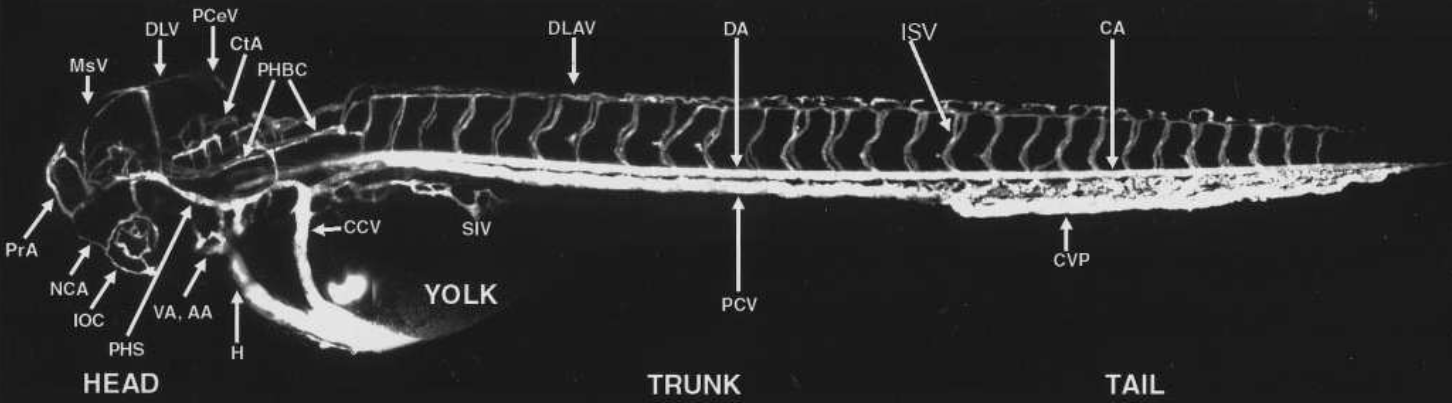
\includegraphics[scale=0.45]{figure/anatomy}
  \end{center}
  \caption[Zebrafish embryo anatomy]{Zebrafish embryo anatomy \cite{isogai01}.}
 \label{anatomy}
\end{figure}
\par

The morphogenesis of the ISV, and CVP involves sprouting, migration, and pruning and can therefore serve as an excellent model for studying angiogenesis.

\section{Challenges}


Current methods analyze images based on intensity and thresholding. These methods perform well on clearly resolved objects against a uniform background but often resort to manual analysis for images that possess information at multiple sizes and heterogeneity across images. To add to the challenge, the images are affected with noise and artifacts. Furthermore, the appearance of zebrafish may vary in intensity, texture, size, and orientation. This problem was brought to attention in a work where zebrafish vasculature became quantifiable only after manual segmentation of the trunk \cite{Tran07}.

Moreover, there is a growing requirement for automated image analysis techniques to process, analyze, and quantify zebrafish images. Meeting such objectives is essential for zebrafish research to reach its full potential in discovery and understanding. Despite the potential of the zebrafish as a model, quantification is still a fledgling field in zebrafish research, primarily due to the lack of tools that can yield objective and quantitative measurements from imaging. From an image processing perspective, a successful algorithm must take into consideration the objectives of the HTS and the content of the images.

All these factors advocate, for automation of as many steps of the analysis as possible. There is an increasing demand for automated image processing to generate quantitative results and to avoid time-consuming manual analysis. According to \cite{Ron13}, the development of dedicated image processing methods has become a serious bottleneck in the full exploitation of the information contained in the acquired image sets. Many custom-made and nongeneric solutions have been developed to answer specific questions. These solutions have an enormous potential to support the analysis of current and future image-based phenotype studies and to avoid parallel developments that tend to \textquotedblleft reinvent the wheel\textquotedblright. We believe that development of a computerized data processing pipeline would be a significant step towards reproducible quantification of phenotypes in large scale or high throughput imaging studies.

Although methods have been developed to process zebrafish images, as the applications of the zebrafish model expands, there is a concurrent demand for a variety of image processing methods. In this work we will focus on the vasculature system of zebrafish, segmenting and developing algorithms for blood vessel development. The vasculature structure is composed of arteries and veins. Blood vessel are highly diverse in length, width, and branching pattern. Significant challenges are associated with blood vessel extraction including, noisy signal, drift in image intensity and poor image contrast.


\section{Research Goal}

%The vascular system is a vital component of all vertebrate animals, supplying oxygen and essential nutrients to everytissue and organ. Zebrafish have a closed circulatory system, and the mechanism of vessel formation are highly similar to those in humans.  It has been suggested that several environmental pollutants could act as vascular disrupting compounds by targeting blood vessel development [3]. A wide range of congenital diseases are associated with blood vessel formation [4], development of the cardiovascular system and associated vascular defects [5], and the adverse effects of exposure to toxic elements during development. 

This work presents a framework of image processing and analysis algorithms that consists of extracting zebrafish, realigning zebrafish embryo images of different orientations, and segmenting, quantifying, and classifying intersegmental vessels (ISV) and caudal vein plexus (CVP). 

Following initial formation of the primitive vasculature by vasculogenesis, most subsequent vessel formation during development takes place via angiogenesis and includes the formation of new vessels by budding growth from, or remodeling of, preexisting vessels. The formation of the ISV and CVP, provides an excellent model for angiogenesis.

ISVs of the trunk are among the first angiogenic vessels to form in all vertebrates. ISVs (fig. \ref{anatomy}) are essential for development and nutrition of the zebrafish embryo. Unlike other vessels, the ISVs are interesting because of the patterned appearance and easy accessibility. Tran et al. \cite{Tran07} has shown that treatment of zebrafish at this early time point had a very strong antiangiogenic effect, causing nearly complete absence of intersegmental vessel growth. The vasculogenic dorsal aorta and posterior cardinal vein were unaffected. Since the intersegmental vessels in zebrafish form by sprouting from the preformed vasculogenic vessels, any compound that disrupts vasculogenesis will also inhibit the growth of angiogenic vessels \cite{Tran07}. All these properties makes ISV one of the most highly investigated vessel in the zebrafish. 

In this work, we have focused on developing an image processing algorithm to automatically segment and quantify ISVs of zebrafish embryos that have been treated by various toxins. The processing pipeline consists of Segmentation, Region Detection, ISV Extraction, ISV refinement, feature quantification and classification. The efficiency of segmentation approach is demonstrated by our experiments of the entire zebrafish vasculature recorded using fluorescence microscopy. The experiments also demonstrate that automated segmentation of ISV is comparable to that of manual segmentation. The quantified features are used to train a linear SVM classifier to identify morphological changes in a dataset consisting of ISV zebrafish embryo images.

Recently, studies have indicated that CVP also undergoes active development, hence providing an additional measure for studying vascular development \cite{Chen05}. The study of the zebrafish CVP and its utilization as a screening assay has not been as prevalent as the ISV, and very few studies have attempted to identify regulators of CVP development. In this work, we study the impact of toxicity on the shape of CVP. Instead of the fine mesh-work of the CVP observed in healthy embryos, treated embryos exhibit the formation of loops in the CVP. %For example, fig \ref{cv} shows the images of healthy and treated zebrafish embryo. 
Previous research has primarily focused on using color, texture \cite{Tran07} and morphological changes \cite{Feng05} for toxicity analysis. Shape information, however, can be another attribute that can be evaluated. A shape descriptor can capture the outline of the shape that other color or texture-based descriptors may not be able to capture.

Hence by quantifying the shape of CVP, and comparing it against that of a healthy embryo, we can identify changes in CVP due to exposure to toxins. Morphological changes due to toxin exposure is modeled based on the proposed gradient weighted co-occurrence histogram of oriented gradients (gCo-HOG). These features are compared to more commonly used histogram of oriented gradients (HOG) features and Co-HOG features that utilizes spatial distribution of neighboring pixels to capture spatial structure. The features are used to train a linear SVM classifier to identify structural changes in a dataset of region of CVP zebrafish embryo images.

We have also presented a study for analyzing effects of Arsenic on overall vasculature development of zebrafish in time-lapse confocal images. We use a transgenic zebrafish that expresses green fluorescent protein (GFP) in the vascular system Tg(Flk1:GFP) to visualize vessel growth in the fish embryo. This transgenic zebrafish line expresses GFP in vascular endothelial cells, which permits real-time imaging of the formation and growth of blood vessels. Time-lapse confocal imaging of embryonic vasculature in the zebrafish is used in conjunction with digital image analysis to monitor and quantify the effect of toxins on vascular development. Imaging captures the dynamics of blood vessel formation over time. In order to quantify these morphological changes, i.e. how much vascular structure has changed over a period of time, it is necessary to compensate for any movements caused by the growing embryo. Thus, in order to record the temporal changes occurring due to vessel growth, it is necessary to establish spatial correspondence between blood vessels that may appear displaced due to embryo movement. Thus quantification of temporal vascular growth can be seen as a problem of image registration. 

The goal of image registration is to align two images, so that common features overlap and differences are emphasized. Image registration has been used widely in the medical field to quantify the influence of changes over time. As an example, registration is required in medicine for comparing computer tomography of patients scan \cite{Betke01}, aligning images from various different modalities to diagnose diseases, etc. Recently, image registration has found application in growth monitoring of tumors and bone \cite{Nielsen97}, \cite{Peter03}. We use a non-rigid registration approach to align images. Non-rigid mapping is based on complete correspondence of images and includes a deformation model as the underlying transformation. We utilize free-form deformation based on B-splines for growth monitoring, and use intensity differences as a similarity measure.

Overall, the methodology presented in this work is quantitative, can be utilized with wide varieties of toxin treated zebrafish, and capable of quantifying changes in fine structure not quantifiable by the human eye. The algorithm automatically processes multiple image files, saves the intermediate image processing results, writes the results in a excel/text format for further statistical analysis. We believe that development of a automated image processing pipeline would be a significant step towards reproducible quantification of zebrafish analysis for HTS. 
%In the past, automatic identification of the applicable region of interes (ROI), and accurate quantification of ROI features has been very challenging.

\section{System Overview}

Zebrafish is a versatile model for vasculature analysis. As its application continues to grow, it is imperative to have an automated image analysis system (fig. \ref{overview}) in place to be able to analyze high throughout data. Obtaining region of interest is the first step for any type of analysis. Multiple zebrafish are imaged in one dish. It is essential to extracts individual zebrafish from image. Our system extracts relevant zebrafish embryo from images. Further, we segment ISV and CVP from embryos. Automated segmentation of ROI opens new opportunities for diversified analysis on zebrafish. 

ISVs are widely used to study toxicology, development, and disease modeling. ISV segmentation is based on multiscale analysis combined with directional information. Multiscale analysis, makes it possible to capture responses from vessels of varying diameter and direction information aids to isolate ISV from other vessels in the region. CVP with its easy accessibility during imaging process, is a potential candidate for research. Realizing its plausible benefits, we have proposed segmentation algorithm based on curvature properties of zebrafish tail.

Although many types of analysis and quantification can be performed on segmented region. Our framework computes morphological properties for quantification of ISV. Shape descriptor is proposed for CVP analysis. Shape descriptor is inspired from Histogram of Gradients. Co-Occurrence of histogram of gradient is combined with gradient information to obtain discriminative representation for CVP region.

Lastly, classification component completes the system. We treat classification as two class binary problem. This system is indicative of healthy embryo vs defective embryo. We demonstrate the validity of our system by analyzing toxin treated data. We used the model to estimate the safe dosage for various chemical. This system can be easily trained to be used for drug modeling, gene expression, etc.

System proposed in this thesis is robust in the manner that each step can be isolated and easily merged with existing or future research. For example, extraction of embryo, ISV and CVP can be effortlessly combined with varied feature extraction methods. 

\begin{landscape}
\begin{figure}[htb] 
 \begin{center}
    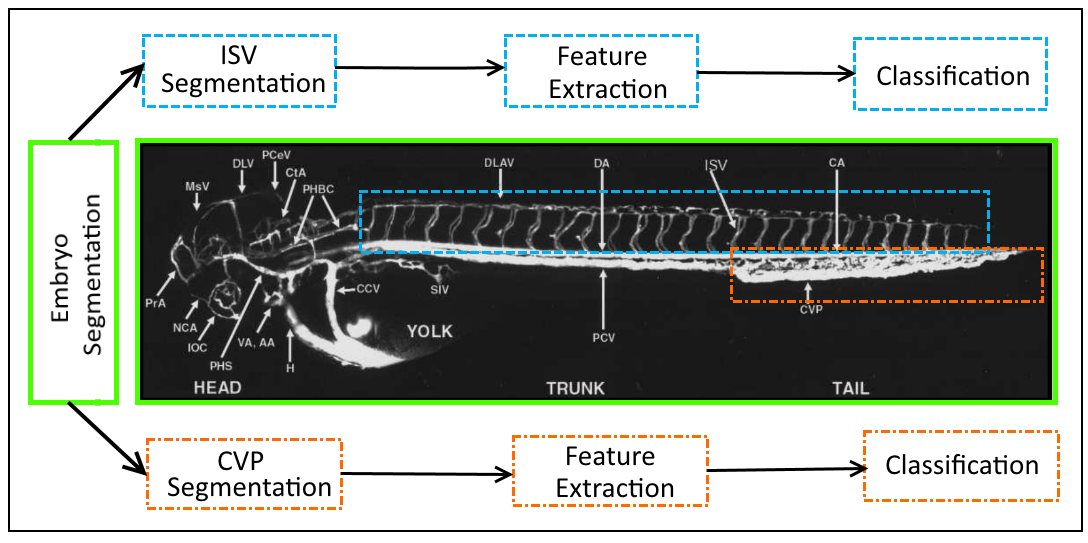
\includegraphics[scale=0.7]{figure/overview.png}
  \end{center}
  \caption[System Overview]{Zebrafish segmentation, feature analysis, classification system}
 \label{overview}
\end{figure}
\end{landscape}



\section{Summary of Contribution}
This thesis studies the image analysis of zebrafish embryo. It makes seven major contributions to this goal:

\begin{itemize}
\item Foremost contribution is the ISV segmentation. There has been many studies indicating viability of using ISV as a model for various application. To our knowledge, automated segmentation of ISV is still largely unstudied problem. In this work we have proposed use of multiscale response and direction information to segment blood vessels.

\item Next is quantification of ISV. We have proposed feature extraction method for ISV morphology, and shown applicability to quantify ISV. Further, we have shown how the features are used for toxicology analysis. 
 
\item Next contribution is segmentation of CVP. CVP is relatively new model as compared to ISV for studying zebrafish. There has been studies showing active molecular development for CVP. Its importance as a model is gaining popularity. CVP segmentation can greatly simplify analysis for HTS. We have proposed an algorithm for CVP segmentation. 

\item In order to utilize shape property of CVP, we have proposed a shape descriptor based on gradient weighted co-occurrence of histogram of gradient. We have proposed to use these descriptors to be able to classify healthy zebrafish embryo, against unhealthy embryos. 

\item We present a toxicology screening system based on lethality rate for ISV and CVP analysis. We used the models derived from morphological properties of ISV and shape properties of CVP to study the effect of increasing dosage on zebrafish in terms of number of zebrafish being impacted with chemicals. Further, this helps us to establish the safe dosage for various chemicals.

\item We studied the vasculature development for time lapse data. This work focuses on capturing temporal vasculature changes in zebrafish. This can work as an initial pass for studying changes in zebrafish development under the influence of chemicals. We have shown utilization of developed algorithms to study arsenic treated zebrafish embryo. 

\item Lastly, the work-flow presented in this thesis is fully automated. The segmentation and analysis of the imaging data is one of the most challenging tasks in automation of the zebrafish applications. Due to lack of robust solutions for this problem, most of the analysis is currently being performed manually. This serves as a huge bottleneck for interpreting data from HTS.

\end{itemize}

\section{Thesis Outline}
The remaining chapters are organized as follows:

\begin{itemize}

\item Chapter \ref{chap:RelatedWork} gives the detail about related work. Related work is clustered according to type of analysis ( automated vs manual).

\item Chapter \ref{chap:seg} presents segmentation algorithm for zebrafish embryo, ISV and CVP. Embryo segmentation is based on region and moment analysis. ISV segmentation uses multiscale property with directional information. CVP segmentation is based on curvature analysis.
 
\item Chapter \ref{chap:feature} describes the features used for quantification of ISV and CVP. We describe our propose algorithm utilizing gradient information with co-occurrence matrix of histogram of gradient. Also, we will discuss time lapse vasculature quantification. 

\item Chapter \ref{chap:results} summarizes approach and our results. We will present results for ISV segmentation, comparing proposed segmentation with manual segmentation. We will also present a classification system for ISV (healthy vs unhealthy), based on its morphological properties. We will also present result for classification system  based on shape properties of CVP. We will describe the toxicology screening system based on modeling ISV and CVP, and how it can be used to derive safe dosage.

\item Lastly, chapter \ref{chap:conclusion} concludes the thesis. We discuss limitations of the work and give guidelines for future work.

\end{itemize}
